\documentclass[12pt]{article}
\usepackage[T1]{fontenc}
\usepackage[T1]{polski}
\usepackage[utf8]{inputenc}
\newcommand{\BibTeX}{{\sc Bib}\TeX} 
\usepackage{graphicx}
\usepackage{amsfonts}
\usepackage{amsmath}
\usepackage{latexsym}
\usepackage{float}

\setlength{\textheight}{21cm}

\title{{\bf Zadanie nr 1 - Generacja sygnału i szumu}\linebreak
Cyfrowe Przetwarzanie Sygnałów}
\author{Dawid Jakubik, 224307 \and Hubert Gawłowski, 224298}
\date{22.04.2021}

\begin{document}
\clearpage\maketitle
\thispagestyle{empty}
\newpage
\setcounter{page}{1}
\section{Cel zadania}

Celem zadania było zapoznanie się z operacjami splotu, filtracji i korelacji sygnałów oraz zaimplementowanie ich rozszerzając tym samym program przygotowany w ramach zadań 1 i 2.

\section{Wstęp teoretyczny}
Podczas pracy nad zadaniem korzystaliśmy z teorii zawartej w intrukcji na platformie Wikamp \cite{instrukcja}. Najważniejsze definicje, jakie trzeba poznać, aby mieć podstawy teoretyczne do zadania dotyczą:
\begin{itemize}
    \item definicji splotu oraz wzoru na niego
    \item definicji korelacji oraz wzoru na korelację bezpośrenią oraz z użyciem splotu
    \item definicji filtracji, filtru dolnoprzepustowego oraz okna prostokątnego, a także wzorów na okna: Hamminga, Hanninga i Blackmana oraz filtrów: śtodkowoprzepustowego i górnoprzepustowego
    \item definicji odpowiedzi impulsowej filtru
\end{itemize}
W ramach zadania, zgodnie z poleceniem poza oknem prostokątnym zaimplementowaliśmy okno Hanninga, a oprócz filtru dolnoprzepustowego został zaimplementowany filtr środkowoprzepustowy.

\section{Eksperymenty i wyniki}

%%%%%%%%%%%%%%%%%%%%%%%%%%%%%%%%%%%%%%%%%%%%%%%%%%%%%%%%%%%%%%%%%%%%%%%%%%%%%%%%%%%%%%%%%%%%%%%%%%%%%%%%%%%%%%%%%
% PODROZDZIA£ PT. EKSPERYMENT NR 1 
%%%%%%%%%%%%%%%%%%%%%%%%%%%%%%%%%%%%%%%%%%%%%%%%%%%%%%%%%%%%%%%%%%%%%%%%%%%%%%%%%%%%%%%%%%%%%%%%%%%%%%%%%%%%%%%%%

\subsection{Splot sygnałów dyskretnych}

Pierwsza pula eksperymentów miała na celu pokazanie splotu sygnałów dyskretnych

\subsubsection{Eksperyment nr 1: Splot sygnałów sinusoidalnych}

W pierwszym eksperymencie dokonaliśmy operacji splotu na dwóch sygnałach sinusoidalnych o następujących parametrach:
\begin{itemize}
    \item Dla sygnału pierwszego: 
    \begin{itemize}
        \item Amplituda: 5
        \item Start w sekundzie: 0
        \item Czas trwania w sekundach: 3
        \item Okres podstawowy: 2
        \item Częstotliwość próbkowania: 70
    \end{itemize}
    \item Dla sygnału drugiego:
    \begin{itemize}
        \item Amplituda: 5
        \item Start w sekundzie: 1
        \item Czas trwania w sekundach: 3
        \item Okres podstawowy: 2
        \item Częstotliwość próbkowania: 70
    \end{itemize}
\end{itemize}
Sygnały wejściowe prezentują się następująco:
\begin{figure}[H]
    \centering
    %\includegraphics{cps_kwantyzacja_z_obcieciem_miary.jpg}
	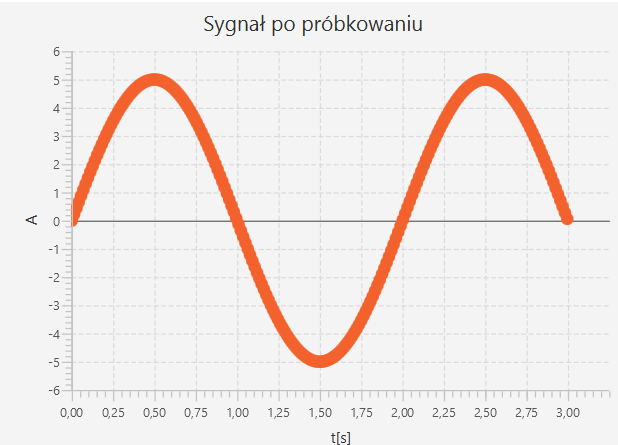
\includegraphics[width=\linewidth]{sygnal_po_probkowaniu_1.1.png}
    \caption{Sygnał nr 1, który zostanie poddany operacji splotu}
    \label{Sygnał_1.1}
\end{figure}

\begin{figure}[H]
    \centering
    %\includegraphics{cps_kwantyzacja_z_obcieciem_miary.jpg}
	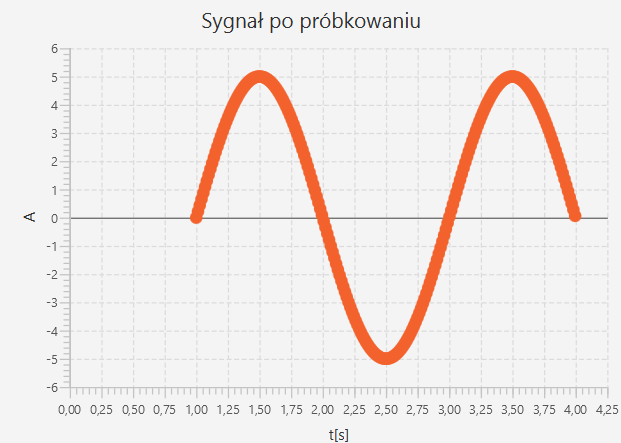
\includegraphics[width=\linewidth]{sygnal_po_probkowaniu_1.2.png}
    \caption{Sygnał nr 2, który zostanie poddany operacji splotu}
    \label{Sygnał_1.2}
\end{figure}

Wynik operacji splotu dwóch powyższych sygnałów przedstawia się następująco
\begin{figure}[H]
    \centering
    %\includegraphics{cps_kwantyzacja_z_obcieciem_miary.jpg}
	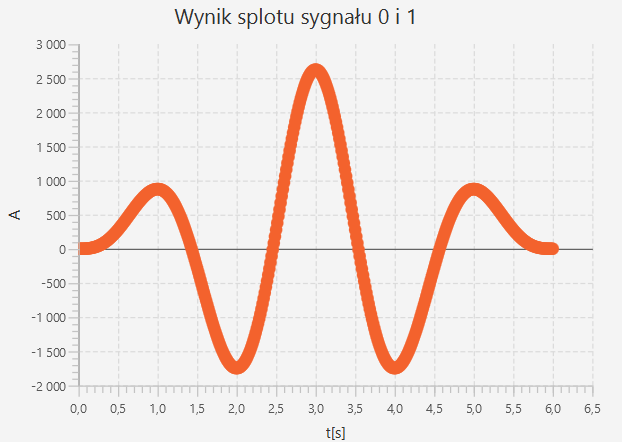
\includegraphics[width=\linewidth]{splot_1.1.png}
    \caption{Wynik operacji splotu sygnałów z rysunków \ref{Sygnał_1.1} i \ref{Sygnał_1.2}}
    \label{Wynik_1.1}
\end{figure}

%%%%%%%%%%%%%%%%%%%%%%%%%%%%%%%%%%%%%%%%%%%%%%%%%%%%%%%%%%%%%%%%%%%%%%%%%%%%%%%%%%%%%%%%%%%%%%%%%%%%%%%%%%%%%%%%%

%%%%%%%%%%%%%%%%%%%%%%%%%%%%%%%%%%%%%%%%%%%%%%%%%%%%%%%%%%%%%%%%%%%%%%%%%%%%%%%%%%%%%%%%%%%%%%%%%%%%%%%%%%%%%%%%%

\subsubsection{Eksperyment nr 2: Splot sygnałów sinusoidalnego wyprostowanego jednopółkowo oraz sygnału trójkątnego}

W kolejnym eksperymencie wykonaliśmy splot na sygnałach sinusoidalnym wyprostowanym jednopółkowym oraz trójkątnym. Sygnały przyjęły następujące parametry:

\begin{itemize}
    \item Dla sygnału pierwszego (sinusoidalnego jednopółkowego): 
    \begin{itemize}
        \item Amplituda: 3
        \item Start w sekundzie: 1
        \item Czas trwania w sekundach: 4
        \item Okres podstawowy: 1
        \item Częstotliwość próbkowania: 50
    \end{itemize}
    \item Dla sygnału drugiego (trójkątnego):
    \begin{itemize}
        \item Amplituda: 2
        \item Start w sekundzie: 1
        \item Czas trwania w sekundach: 4
        \item Okres podstawowy: 3
        \item Współczynnik wypełnienia: 0.4
        \item Częstotliwość próbkowania: 50
    \end{itemize}
\end{itemize}
Sygnały wejściowe prezentują się następująco:
\begin{figure}[H]
    \centering
    %\includegraphics{cps_kwantyzacja_z_obcieciem_miary.jpg}
	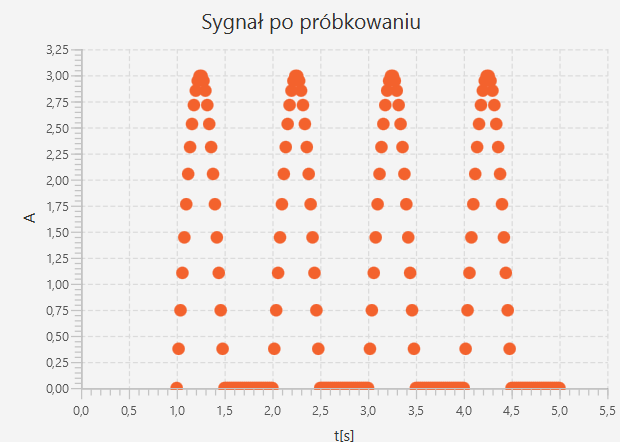
\includegraphics[width=\linewidth]{sygnal_po_probkowaniu_2.1.png}
    \caption{Sygnał nr 1, który zostanie poddany operacji splotu}
    \label{Sygnał_2.1}
\end{figure}

\begin{figure}[H]
    \centering
    %\includegraphics{cps_kwantyzacja_z_obcieciem_miary.jpg}
	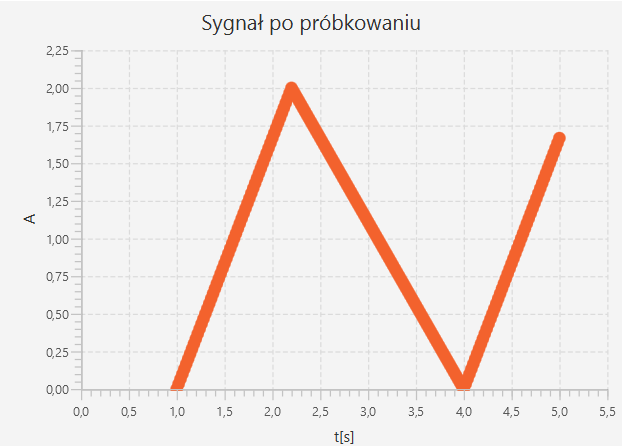
\includegraphics[width=\linewidth]{sygnal_po_probkowaniu_2.2.png}
    \caption{Sygnał nr 2, który zostanie poddany operacji splotu}
    \label{Sygnał_2.2}
\end{figure}

Wynik operacji splotu dwóch powyższych sygnałów przedstawia się następująco
\begin{figure}[H]
    \centering
    %\includegraphics{cps_kwantyzacja_z_obcieciem_miary.jpg}
	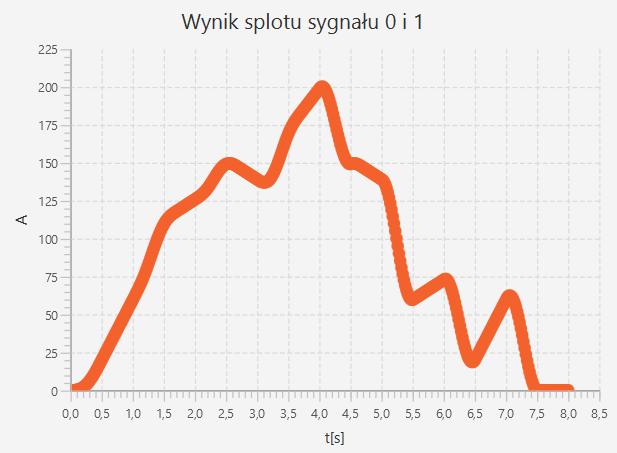
\includegraphics[width=\linewidth]{splot_2.1.png}
    \caption{Wynik operacji splotu sygnałów z rysunków \ref{Sygnał_2.1} i \ref{Sygnał_2.2}}
    \label{Wynik_2.1}
\end{figure}

%%%%%%%%%%%%%%%%%%%%%%%%%%%%%%%%%%%%%%%%%%%%%%%%%%%%%%%%%%%%%%%%%%%%%%%%%%%%%%%%%%%%%%%%%%%%%%%%%%%%%%%%%%%%%%%%%

%%%%%%%%%%%%%%%%%%%%%%%%%%%%%%%%%%%%%%%%%%%%%%%%%%%%%%%%%%%%%%%%%%%%%%%%%%%%%%%%%%%%%%%%%%%%%%%%%%%%%%%%%%%%%%%%%

\subsubsection{Eksperyment nr 3:  Splot sygnałów trójkątnego oraz sinusoidalnego wyprostowanego jednopółkowo}
W kolejnym eksperymencie przeprowadziliśmy splot na takich samych sygnałach jak w eksperymencie powyżej, jednak zmieniliśmy kolejność sygnałów - w tym przypadku sygnałem nr 1 będzie sygnał trójkątny, a sygnałem nr 2 - sygnał sinusoidalny jednopółkowy. Celem tego eksperymentu jest zbadanie, czy wzór (2) podany w instrukcji do zadania \cite{instrukcja} jest przemienny tzn. czy (h*x)(n) da nam ten sam wynik, co (x*h)(n). Tak więc - podsumowując do eksperymentów wykorzystamy następujące z następującymi parametrami:
\begin{itemize}
    \item Dla sygnału pierwszego (trójkątnego):
    \begin{itemize}
        \item Amplituda: 2
        \item Start w sekundzie: 1
        \item Czas trwania w sekundach: 4
        \item Okres podstawowy: 3
        \item Współczynnik wypełnienia: 0.4
        \item Częstotliwość próbkowania: 50
    \end{itemize}
    \item Dla sygnału drugiego (sinusoidalnego jednopółkowego): 
    \begin{itemize}
        \item Amplituda: 3
        \item Start w sekundzie: 1
        \item Czas trwania w sekundach: 4
        \item Okres podstawowy: 1
        \item Częstotliwość próbkowania: 50
    \end{itemize}
\end{itemize}
Sygnały wejściowe prezentują się następująco:
\begin{figure}[H]
    \centering
    %\includegraphics{cps_kwantyzacja_z_obcieciem_miary.jpg}
	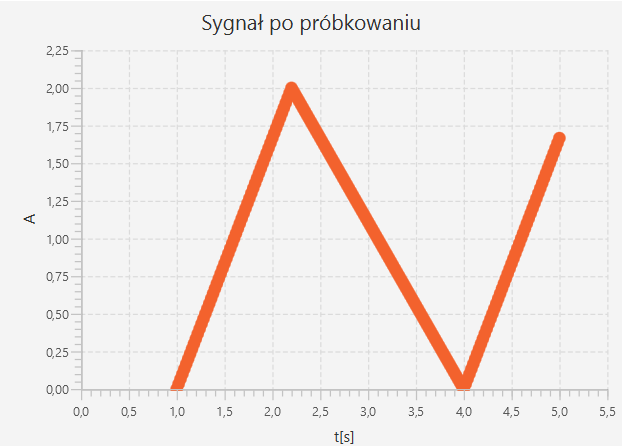
\includegraphics[width=\linewidth]{sygnal_po_probkowaniu_2.2.png}
    \caption{Sygnał nr 1, który zostanie poddany operacji splotu}
    \label{Sygnał_3.1}
\end{figure}

\begin{figure}[H]
    \centering
    %\includegraphics{cps_kwantyzacja_z_obcieciem_miary.jpg}
	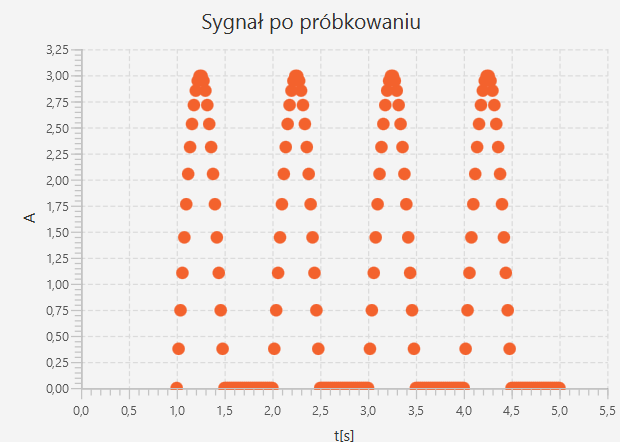
\includegraphics[width=\linewidth]{sygnal_po_probkowaniu_2.1.png}
    \caption{Sygnał nr 2, który zostanie poddany operacji splotu}
    \label{Sygnał_3.2}
\end{figure}

Wynik operacji splotu dwóch powyższych sygnałów przedstawia się następująco
\begin{figure}[H]
    \centering
    %\includegraphics{cps_kwantyzacja_z_obcieciem_miary.jpg}
	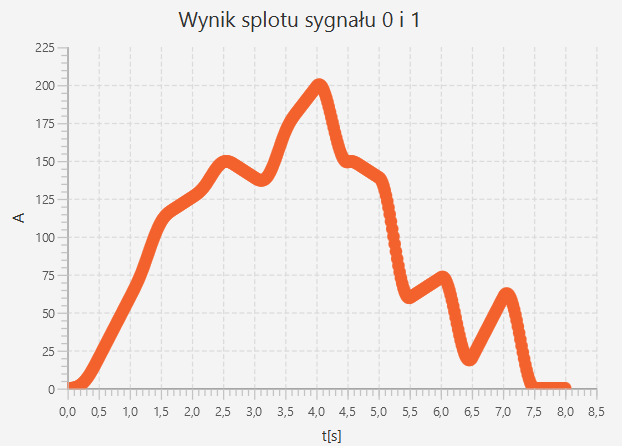
\includegraphics[width=\linewidth]{splot_3.1.png}
    \caption{Wynik operacji splotu sygnałów z rysunków \ref{Sygnał_3.1} i \ref{Sygnał_3.2}}
    \label{Wynik_3.1}
\end{figure}

%%%%%%%%%%%%%%%%%%%%%%%%%%%%%%%%%%%%%%%%%%%%%%%%%%%%%%%%%%%%%%%%%%%%%%%%%%%%%%%%%%%%%%%%%%%%%%%%%%%%%%%%%%%%%%%%%

%%%%%%%%%%%%%%%%%%%%%%%%%%%%%%%%%%%%%%%%%%%%%%%%%%%%%%%%%%%%%%%%%%%%%%%%%%%%%%%%%%%%%%%%%%%%%%%%%%%%%%%%%%%%%%%%%

\subsubsection{Eksperyment nr 4: Splot sygnałów prostokątnego i sinusoidalnego wyprostowanego dwupółkowo}
W tym eksperymencie dokonaliśmy splotu na sygnałach prostokątym oraz sinusoidalnym dwupółkowym o następujących parametrach:
\begin{itemize}
    \item Dla sygnału pierwszego (prostokątnego):
    \begin{itemize}
        \item Amplituda: 4
        \item Start w sekundzie: 0
        \item Czas trwania w sekundach: 4
        \item Okres podstawowy: 2
        \item Współczynnik wypełnienia: 0.6
        \item Częstotliwość próbkowania: 10
    \end{itemize}
    \item Dla sygnału drugiego (sinusoidalnego dwupółkowego): 
    \begin{itemize}
        \item Amplituda: 1 
        \item Start w sekundzie: 0 
        \item Czas trwania w sekundach: 4
        \item Okres podstawowy: 4
        \item Częstotliwość próbkowania: 20
    \end{itemize}
\end{itemize}
Sygnały wejściowe prezentują się następująco:
\begin{figure}[H]
    \centering
    %\includegraphics{cps_kwantyzacja_z_obcieciem_miary.jpg}
	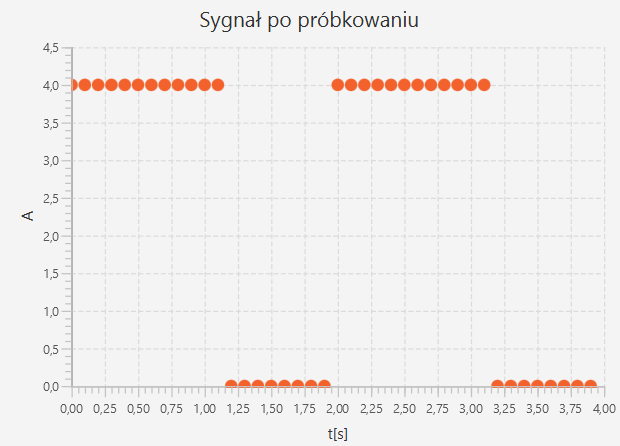
\includegraphics[width=\linewidth]{sygnal_po_probkowaniu_4.1.png}
    \caption{Sygnał nr 1, który zostanie poddany operacji splotu}
    \label{Sygnał_4.1}
\end{figure}

\begin{figure}[H]
    \centering
    %\includegraphics{cps_kwantyzacja_z_obcieciem_miary.jpg}
	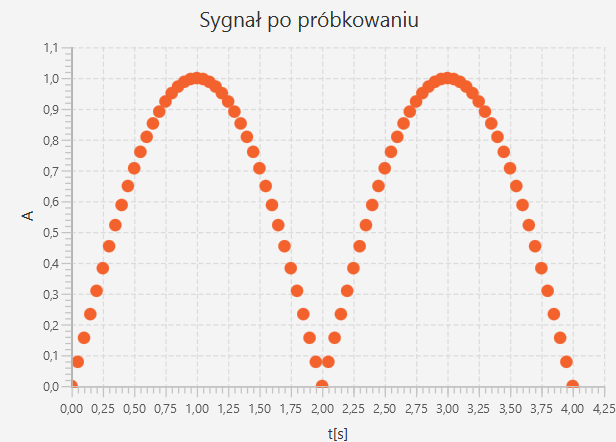
\includegraphics[width=\linewidth]{sygnal_po_probkowaniu_4.2.png}
    \caption{Sygnał nr 2, który zostanie poddany operacji splotu}
    \label{Sygnał_4.2}
\end{figure}

Wynik operacji splotu dwóch powyższych sygnałów przedstawia się następująco
\begin{figure}[H]
    \centering
    %\includegraphics{cps_kwantyzacja_z_obcieciem_miary.jpg}
	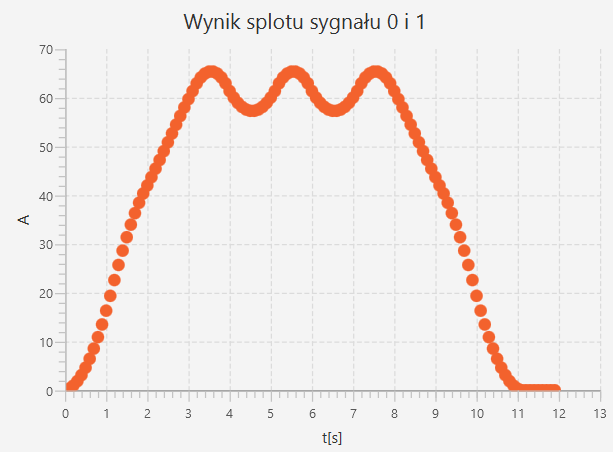
\includegraphics[width=\linewidth]{splot_4.1.png}
    \caption{Wynik operacji splotu sygnałów z rysunków \ref{Sygnał_4.1} i \ref{Sygnał_4.2}}
    \label{Wynik_4.1}
\end{figure}





%%%%%%%%%%%%%%%%%%%%%%%%%%%%%%%%%%%%%%%%%%%%%%%%%%%%%%%%%%%%%%%%%%%%%%%%%%%%%%%%%%%%%%%%%%%%%%%%%%%%%%%%%%%%%%%%%
%%%%%%%%%%%%%%%%%%%%%%%%%%%%%%%%%%%%%%%%%%%%%%%%%%%%%%%%%%%%%%%%%%%%%%%%%%%%%%%%%%%%%%%%%%%%%%%%%%%%%%%%%%%%%%%%%

%%%%%%%%%%%%%%%%%%%%%%%%%%%%%%%%%%%%%%%%%%%%%%%%%%%%%%%%%%%%%%%%%%%%%%%%%%%%%%%%%%%%%%%%%%%%%%%%%%%%%%%%%%%%%%%%%
%%%%%%%%%%%%%%%%%%%%%%%%%%%%%%%%%%%%%%%%%%%%%%%%%%%%%%%%%%%%%%%%%%%%%%%%%%%%%%%%%%%%%%%%%%%%%%%%%%%%%%%%%%%%%%%%%

\subsection{Korelacja sygnałów dyskretnych}

W celu lepszego zwizualizowania podobieństw/różnic pomiędzy korelacją, a splotem eksperymenty dla korelacji postanowiliśmy wykonać wykorzystując te same sygnały wjeściowe, które mimo wszystko przedstawimy jeszcze raz w ramach eksperymentów.

\subsubsection{Eksperyment nr 5: Korelacja bezpośrednia sygnałów sinusoidalnych}
W pierwszym eksperymencie dotyczącym korelacji dokonaliśmy operacji korelacji bezpośredniej na dwóch sygnałach sinusoidalnych o następujących parametrach:
\begin{itemize}
    \item Dla sygnału pierwszego: 
    \begin{itemize}
        \item Amplituda: 5
        \item Start w sekundzie: 0
        \item Czas trwania w sekundach: 3
        \item Okres podstawowy: 2
        \item Częstotliwość próbkowania: 70
    \end{itemize}
    \item Dla sygnału drugiego:
    \begin{itemize}
        \item Amplituda: 5
        \item Start w sekundzie: 1
        \item Czas trwania w sekundach: 3
        \item Okres podstawowy: 2
        \item Częstotliwość próbkowania: 70
    \end{itemize}
\end{itemize}
Sygnały wejściowe prezentują się następująco:
\begin{figure}[H]
    \centering
    %\includegraphics{cps_kwantyzacja_z_obcieciem_miary.jpg}
	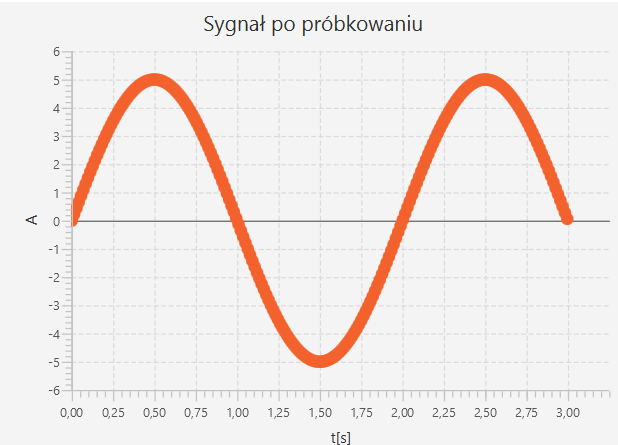
\includegraphics[width=\linewidth]{sygnal_po_probkowaniu_1.1.png}
    \caption{Sygnał nr 1, który zostanie poddany operacji splotu}
    \label{Sygnał_5.1}
\end{figure}

\begin{figure}[H]
    \centering
    %\includegraphics{cps_kwantyzacja_z_obcieciem_miary.jpg}
	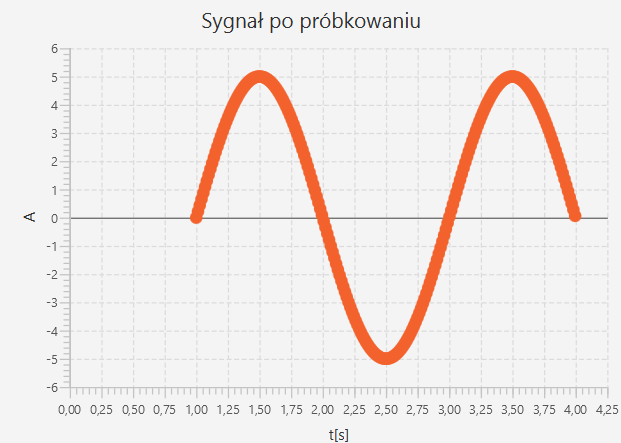
\includegraphics[width=\linewidth]{sygnal_po_probkowaniu_1.2.png}
    \caption{Sygnał nr 2, który zostanie poddany operacji splotu}
    \label{Sygnał_5.2}
\end{figure}

Wynik operacji korelacji dwóch powyższych sygnałów przedstawia się następująco
\begin{figure}[H]
    \centering
    %\includegraphics{cps_kwantyzacja_z_obcieciem_miary.jpg}
	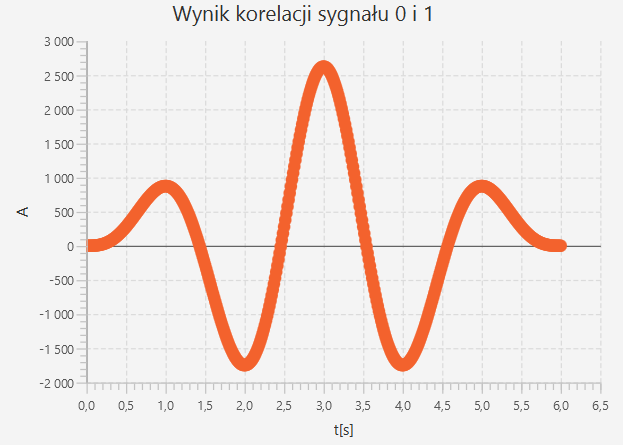
\includegraphics[width=\linewidth]{Korelacja_5.1.png}
    \caption{Wynik operacji korelacji sygnałów z rysunków \ref{Sygnał_5.1} i \ref{Sygnał_5.2}}
    \label{Wynik_5.1}
\end{figure}

%%%%%%%%%%%%%%%%%%%%%%%%%%%%%%%%%%%%%%%%%%%%%%%%%%%%%%%%%%%%%%%%%%%%%%%%%%%%%%%%%%%%%%%%%%%%%%%%%%%%%%%%%%%%%%%%%

%%%%%%%%%%%%%%%%%%%%%%%%%%%%%%%%%%%%%%%%%%%%%%%%%%%%%%%%%%%%%%%%%%%%%%%%%%%%%%%%%%%%%%%%%%%%%%%%%%%%%%%%%%%%%%%%%
\subsubsection{Eksperyment nr 6: Korelacja bezpośrednia sygnałów sinusoidalnego wyprostowanego jednopółkowo oraz sygnału trójkątnego}

W kolejnym eksperymencie wykonaliśmy korelacje bezpośrednią na sygnałach sinusoidalnym wyprostowanym jednopółkowym oraz trójkątnym. Sygnały przyjęły następujące parametry:

\begin{itemize}
    \item Dla sygnału pierwszego (sinusoidalnego jednopółkowego): 
    \begin{itemize}
        \item Amplituda: 3
        \item Start w sekundzie: 1
        \item Czas trwania w sekundach: 4
        \item Okres podstawowy: 1
        \item Częstotliwość próbkowania: 50
    \end{itemize}
    \item Dla sygnału drugiego (trójkątnego):
    \begin{itemize}
        \item Amplituda: 2
        \item Start w sekundzie: 1
        \item Czas trwania w sekundach: 4
        \item Okres podstawowy: 3
        \item Współczynnik wypełnienia: 0.4
        \item Częstotliwość próbkowania: 50
    \end{itemize}
\end{itemize}
Sygnały wejściowe prezentują się następująco:
\begin{figure}[H]
    \centering
    %\includegraphics{cps_kwantyzacja_z_obcieciem_miary.jpg}
	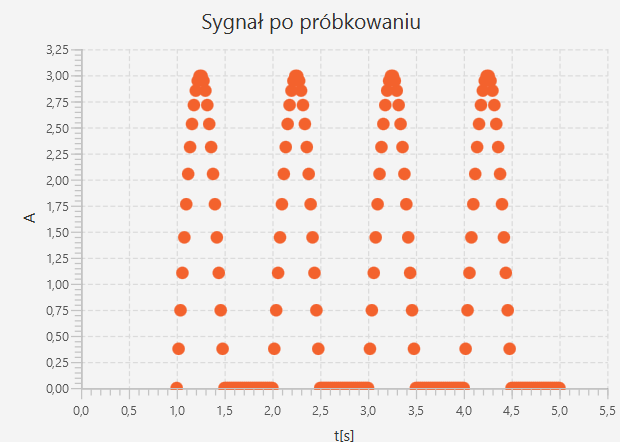
\includegraphics[width=\linewidth]{sygnal_po_probkowaniu_2.1.png}
    \caption{Sygnał nr 1, który zostanie poddany operacji splotu}
    \label{Sygnał_6.1}
\end{figure}

\begin{figure}[H]
    \centering
    %\includegraphics{cps_kwantyzacja_z_obcieciem_miary.jpg}
	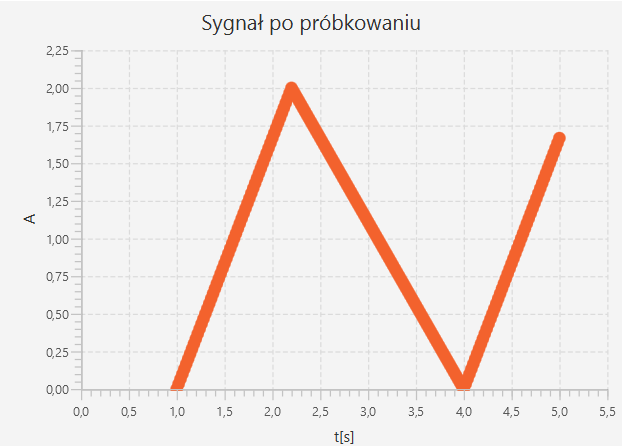
\includegraphics[width=\linewidth]{sygnal_po_probkowaniu_2.2.png}
    \caption{Sygnał nr 2, który zostanie poddany operacji splotu}
    \label{Sygnał_6.2}
\end{figure}

Wynik operacji korelacji bezpośredniej dwóch powyższych sygnałów przedstawia się następująco
\begin{figure}[H]
    \centering
    %\includegraphics{cps_kwantyzacja_z_obcieciem_miary.jpg}
	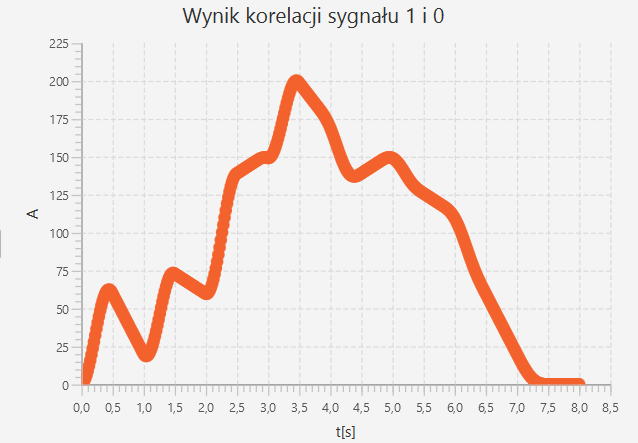
\includegraphics[width=\linewidth]{Korelacja_61.png}
    \caption{Wynik operacji korelacji sygnałów z rysunków \ref{Sygnał_6.1} i \ref{Sygnał_6.2}}
    \label{Wynik_6.1}
\end{figure}
%%%%%%%%%%%%%%%%%%%%%%%%%%%%%%%%%%%%%%%%%%%%%%%%%%%%%%%%%%%%%%%%%%%%%%%%%%%%%%%%%%%%%%%%%%%%%%%%%%%%%%%%%%%%%%%%%

%%%%%%%%%%%%%%%%%%%%%%%%%%%%%%%%%%%%%%%%%%%%%%%%%%%%%%%%%%%%%%%%%%%%%%%%%%%%%%%%%%%%%%%%%%%%%%%%%%%%%%%%%%%%%%%%%
\subsubsection{Eksperyment nr 7: Korelacja bezpośrednia sygnałów trójkątnego oraz sinusoidalnego wyprostowanego jednopółkowo}
W kolejnym eksperymencie przeprowadziliśmy korelację bezpośrednią na takich samych sygnałach jak w eksperymencie powyżej, jednak zmieniliśmy kolejność sygnałów - w tym przypadku sygnałem nr 1 będzie sygnał trójkątny, a sygnałem nr 2 - sygnał sinusoidalny jednopółkowy. Celem tego eksperymentu jest zbadanie, czy wzór (2) podany w instrukcji do zadania \cite{instrukcja} jest przemienny tzn. czy (h*x)(n) da nam ten sam wynik, co (x*h)(n). Tak więc - podsumowując do eksperymentów wykorzystamy następujące z następującymi parametrami:
\begin{itemize}
    \item Dla sygnału pierwszego (trójkątnego):
    \begin{itemize}
        \item Amplituda: 2
        \item Start w sekundzie: 1
        \item Czas trwania w sekundach: 4
        \item Okres podstawowy: 3
        \item Współczynnik wypełnienia: 0.4
        \item Częstotliwość próbkowania: 50
    \end{itemize}
    \item Dla sygnału drugiego (sinusoidalnego jednopółkowego): 
    \begin{itemize}
        \item Amplituda: 3
        \item Start w sekundzie: 1
        \item Czas trwania w sekundach: 4
        \item Okres podstawowy: 1
        \item Częstotliwość próbkowania: 50
    \end{itemize}
\end{itemize}
Sygnały wejściowe prezentują się następująco:
\begin{figure}[H]
    \centering
    %\includegraphics{cps_kwantyzacja_z_obcieciem_miary.jpg}
	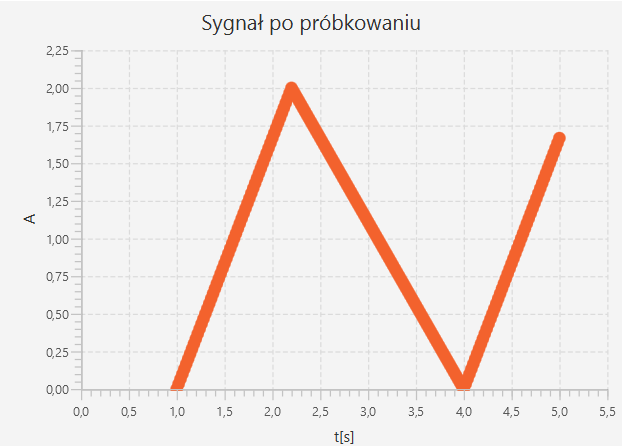
\includegraphics[width=\linewidth]{sygnal_po_probkowaniu_2.2.png}
    \caption{Sygnał nr 1, który zostanie poddany operacji splotu}
    \label{Sygnał_7.1}
\end{figure}

\begin{figure}[H]
    \centering
    %\includegraphics{cps_kwantyzacja_z_obcieciem_miary.jpg}
	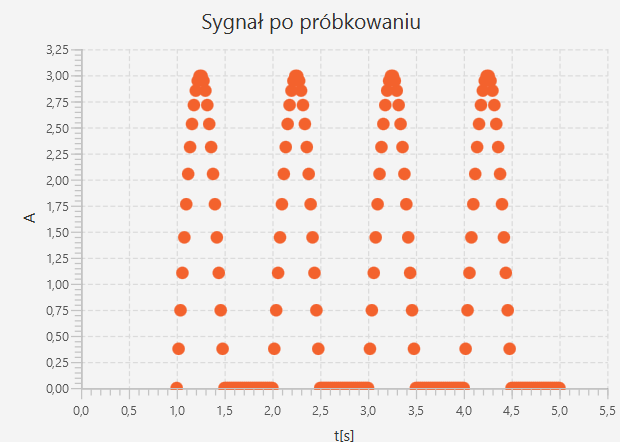
\includegraphics[width=\linewidth]{sygnal_po_probkowaniu_2.1.png}
    \caption{Sygnał nr 2, który zostanie poddany operacji splotu}
    \label{Sygnał_7.2}
\end{figure}

Wynik operacji korelacji bezpośredniej dwóch powyższych sygnałów przedstawia się następująco
\begin{figure}[H]
    \centering
    %\includegraphics{cps_kwantyzacja_z_obcieciem_miary.jpg}
	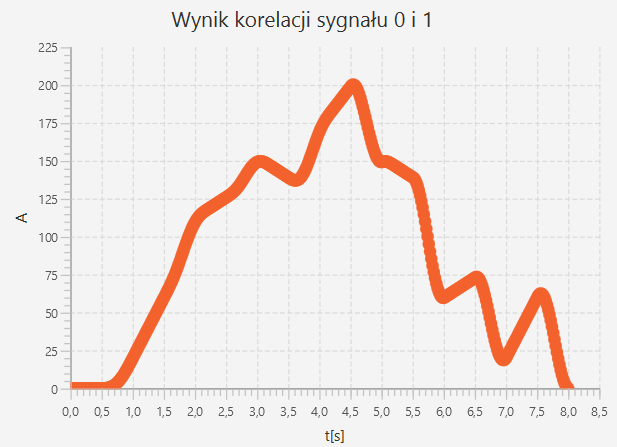
\includegraphics[width=\linewidth]{Korelacja_7.1.png}
    \caption{Wynik operacji korelacji sygnałów z rysunków \ref{Sygnał_7.1} i \ref{Sygnał_7.2}}
    \label{Wynik_7.1}
\end{figure}
%%%%%%%%%%%%%%%%%%%%%%%%%%%%%%%%%%%%%%%%%%%%%%%%%%%%%%%%%%%%%%%%%%%%%%%%%%%%%%%%%%%%%%%%%%%%%%%%%%%%%%%%%%%%%%%%%

%%%%%%%%%%%%%%%%%%%%%%%%%%%%%%%%%%%%%%%%%%%%%%%%%%%%%%%%%%%%%%%%%%%%%%%%%%%%%%%%%%%%%%%%%%%%%%%%%%%%%%%%%%%%%%%%%
\subsubsection{Eksperyment nr 8: Korelacja z wykorzystaniem splotu sygnałów prostokątnego i sinusoidalnego wyprostowanego dwupółkowo}
W tym eksperymencie dokonaliśmy korelacji z użciem splotu na sygnałach prostokątym oraz sinusoidalnym dwupółkowym o następujących parametrach:
\begin{itemize}
    \item Dla sygnału pierwszego (prostokątnego):
    \begin{itemize}
        \item Amplituda: 4
        \item Start w sekundzie: 0
        \item Czas trwania w sekundach: 4
        \item Okres podstawowy: 2
        \item Współczynnik wypełnienia: 0.6
        \item Częstotliwość próbkowania: 10
    \end{itemize}
    \item Dla sygnału drugiego (sinusoidalnego dwupółkowego): 
    \begin{itemize}
        \item Amplituda: 1 
        \item Start w sekundzie: 0 
        \item Czas trwania w sekundach: 4
        \item Okres podstawowy: 4
        \item Częstotliwość próbkowania: 20
    \end{itemize}
\end{itemize}
Sygnały wejściowe prezentują się następująco:
\begin{figure}[H]
    \centering
    %\includegraphics{cps_kwantyzacja_z_obcieciem_miary.jpg}
	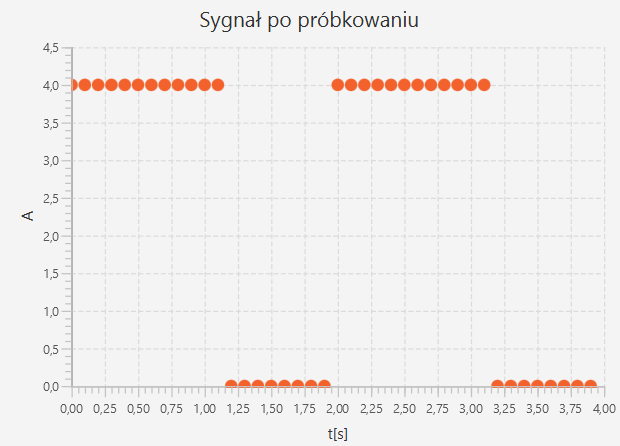
\includegraphics[width=\linewidth]{sygnal_po_probkowaniu_4.1.png}
    \caption{Sygnał nr 1, który zostanie poddany operacji splotu}
    \label{Sygnał_8.1}
\end{figure}

\begin{figure}[H]
    \centering
    %\includegraphics{cps_kwantyzacja_z_obcieciem_miary.jpg}
	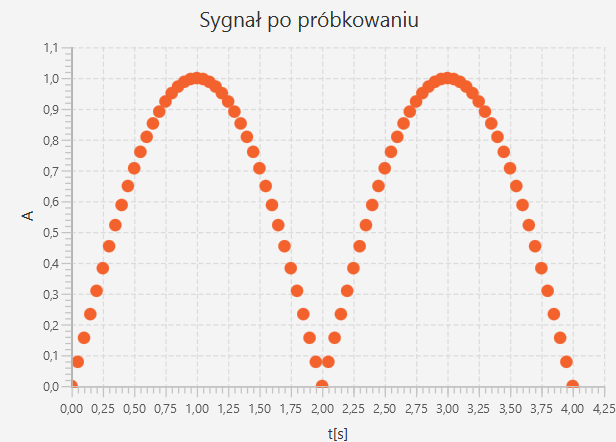
\includegraphics[width=\linewidth]{sygnal_po_probkowaniu_4.2.png}
    \caption{Sygnał nr 2, który zostanie poddany operacji splotu}
    \label{Sygnał_8.2}
\end{figure}

Wynik operacji korelacji z wykorzystaniem splotu dwóch powyższych sygnałów przedstawia się następująco
\begin{figure}[H]
    \centering
    %\includegraphics{cps_kwantyzacja_z_obcieciem_miary.jpg}
	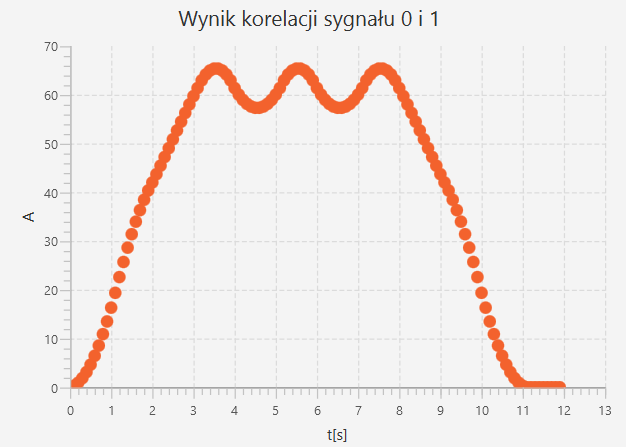
\includegraphics[width=\linewidth]{Korelacja_581.png}
    \caption{Wynik operacji korelacji z wykorzystaniem splotu sygnałów z rysunków \ref{Sygnał_8.1} i \ref{Sygnał_8.2}}
    \label{Wynik_8.1}
\end{figure}

\subsection{Eksperyment nr 9: Filtracja sygnału sinusoidalnego} 
W ramach tego eksperymentu poddaliśmy poniższy sygnał sinusoidalny filtracjom. Podczs obu filtracji przyjęliśmy
\begin{itemize}
	\item rząd filtru: 25
	\item Częstotliwość odcięcia: 10Hz
	\item Częstotliwość próbkowania sygnału: 80Hz
\end{itemize}

\begin{figure}[H]
	\centering
	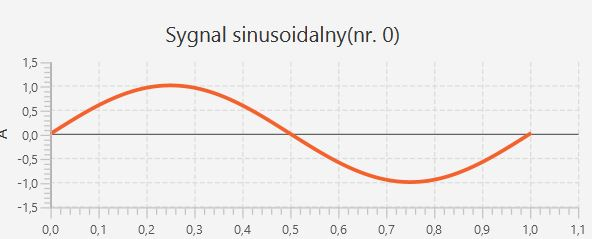
\includegraphics[width=\linewidth]{sinus-wejscie}
	\caption{Sygnał sinusoidalny}
	\label{}
\end{figure}

Poniżej przedstawiony został filtr dolnoprzepustowy z oknem Hanninga oraz wynik filtracji.
\begin{figure}[H]
	\centering
	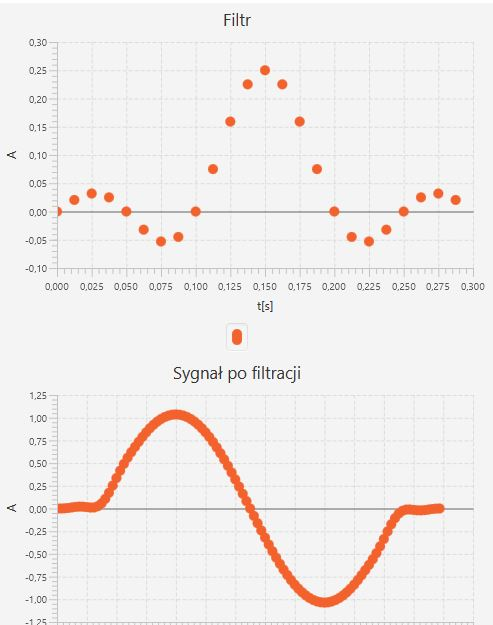
\includegraphics[width=\linewidth]{filtr-dolnoprzep-hannin}
	\caption{Filtr oraz wynik filtracji dla filtra dolnoprzepustowego i zastosowania okna Hanninga}
	\label{}
\end{figure}


Poniżej przedstawiony został filtr pasmowy z oknem prostokątnym oraz wynik filtracji.
\begin{figure}[H]
	\centering
	\includegraphics[width=\linewidth]{filtr-pasmowy-prost}
	\caption{Filtr oraz wynik filtracji dla filtra pasmowego i zastosowania okna prostokątnego}
	\label{}
\end{figure}
%%%%%%%%%%%%%%%%%%%%%%%%%%%%%%%%%%%%%%%%%%%%%%%%%%%%%%%%%%%%%%%%%%%%%%%%%%%%%%%%%%%%%%%%%%%%%%%%%%%%%%%%%%%%%%%%%

%%%%%%%%%%%%%%%%%%%%%%%%%%%%%%%%%%%%%%%%%%%%%%%%%%%%%%%%%%%%%%%%%%%%%%%%%%%%%%%%%%%%%%%%%%%%%%%%%%%%%%%%%%%%%%%%%
\section{Wnioski}
Program umożliwia generowanie wykresów będącymi wynikami operacji splotu, korelacji oraz filtracji.
\subsection{Splot sygnałów dyskretnych}
Pierwsza pula eksperymentów polegała na splocie sygnałów dyskretnych. W eksperymencie nr 1 dokonaliśmy operacji splotu na takich samych sygnałach sinusoidalnych, przesuniętych w czasie o 1 s. Wynik operacji splotu jest zgodny z założeniami. Sygnał wynikowy ma okres równy sumie okresów obu sygnałów. Pozwala nam to wysnuć wniosek, że przesunięcie w czasie nie ma wpływu na operacje splotu. W eksperymencie 2, w którym dokonaliśmy operacji splotu dla sygnałów sinusoidalnego wyprostowanego jednopółkowo oraz trójkątnego wyniki również wydają się logiczne i sensowne. Długość trwania sygnału splotu odpowiada sumie długości trwania sygnałów wejściowych, a maksymalną wartość splot przyjmuje dokładnie w połowie czasu trwania. Następny eksperyment (nr 3) dowodzi, że operacja splotu jest przemienna tzn. bez względu, który sygnał przyjmiemy jako h, a który jako x we wzorze na splot \cite{instrukcja} - wynik będzie taki sam. Eksperyment 4 przeprowadziliśmy dla typów sygnałów, dla których wcześniej nie przeprowadzaliśmy eksperymentów oraz z zdecydowanie mniejszą (i różną od siebie) częstotliwością próbkowania. Wynik pokazuje, że przy operacji splotu częstotliwość próbkowania obu sygnałów dyskretnych nie musi być taka sama.

\subsection{Korelacja sygnałów dyskretnych}
Druga pula eksperymentów polegała na pokazaniu operacji korelacji sygnałów dyskretnych. Eksperymenty przeprowadziliśmy dla takich samych sygnałów jak przy operacji splotu. Pierwszy z eksperymentów wykonany na sygnałach sinusoidalnych (a więc sygnałach symetrycznych) dał wynik dokładnie taki sam jak w przypadku splotu dla tych sygnałów. Różnice w rezultacie, jeśli porównamy go z operacją splotu dla analogicznych sygnałów możemy zaobserwować w eksperymencie nr 6. Co ciekawe, jest to po prostu odbicie lustrzane względem prostej y = 4 (środek wykresu). Eksperyment 7 pokazał nam, że w przypadku korelacji parametry x i h ze wzoru zawartego w \cite{instrukcja} nie mogą być stosowane zamiennie. W eksperymencie 8 pokazaliśmy korelacji z wykorzystaniem splotu. Wynik nie może dziwić - jest on po prostu wykresem powstałym w wyniku splotu dwóch sygnałów, a więc powstaje wykres taki sam jak w eksperymencie nr 4. 

\subsection{Filtracja sygnałów dyskretnych}
Podczas procesu filtracji skupiliśmy się przede wszystkim na uzyskaniu optymalnej odpowiedzi impulsowej, którą potem należy wykorzystać w operacji splotu, aby uzyskać sygnał przefiltrowany. Uważamy, że okno Hanninga daje zdecydowanie lepsze i dokładniejsze rezultaty od okna prostokątnego. Co do filtra dolnoprzepustowego i środkowoprzepustowego wydaje nam się, że ciężko jednoznacznie stwierdzić, który z nich jest "lepszy". Uważamy, że ich zastosowanie należy uzależnić od konkretnego przypadku - w niektórych lepiej sprawdzi się filtr dolnoprzpustowy, a w innych - średnioprzepustowy.

\subsection{Ostateczne najważniejsze wnioski}
\begin{itemize}
    \item Operacje korelacji i splotu są do siebie bardzo podobne, a w niektórych przypadkach dają w wyniku ten sam rezultat. Ponadto można zrealizować korelację w oparciu o splot.
    \item Zastosowanie funkcji okna pozwala zwiększyć efektywność filtru.
    \item Im większy rząd filtra, tym jakość filtracji lepsza
    \item Metoda filtrów SOI zastosowana w zadaniu generuje zakłócenia na krańcach odfiltrowanego sygnału.
\end{itemize}
%%%%%%%%%%%%%%%%%%%%%%%%%%%%%%%%%%%%%%%%%%%%%%%%%%%%%%%%%%%%%%%%%%%%%%%%%%%%%%%%%%%%%%%%%%%%%%%%%%%%%%%%%%%%%%%%%
% BIBLIOGRAFIA
%%%%%%%%%%%%%%%%%%%%%%%%%%%%%%%%%%%%%%%%%%%%%%%%%%%%%%%%%%%%%%%%%%%%%%%%%%%%%%%%%%%%%%%%%%%%%%%%%%%%%%%%%%%%%%%%%
\begin{thebibliography}{}
\bibitem{instrukcja} Instrukcja do zadania 3 na stronie przedmiotu. [przeglądany 26.05.2021], Dostępny w: https://ftims.edu.p.lodz.pl/pluginfile.php/14039/mod\_resource/content/1/zad3.pdf


\end{thebibliography}



\end{document}
